\begin{figure}[!htbp]
\centering
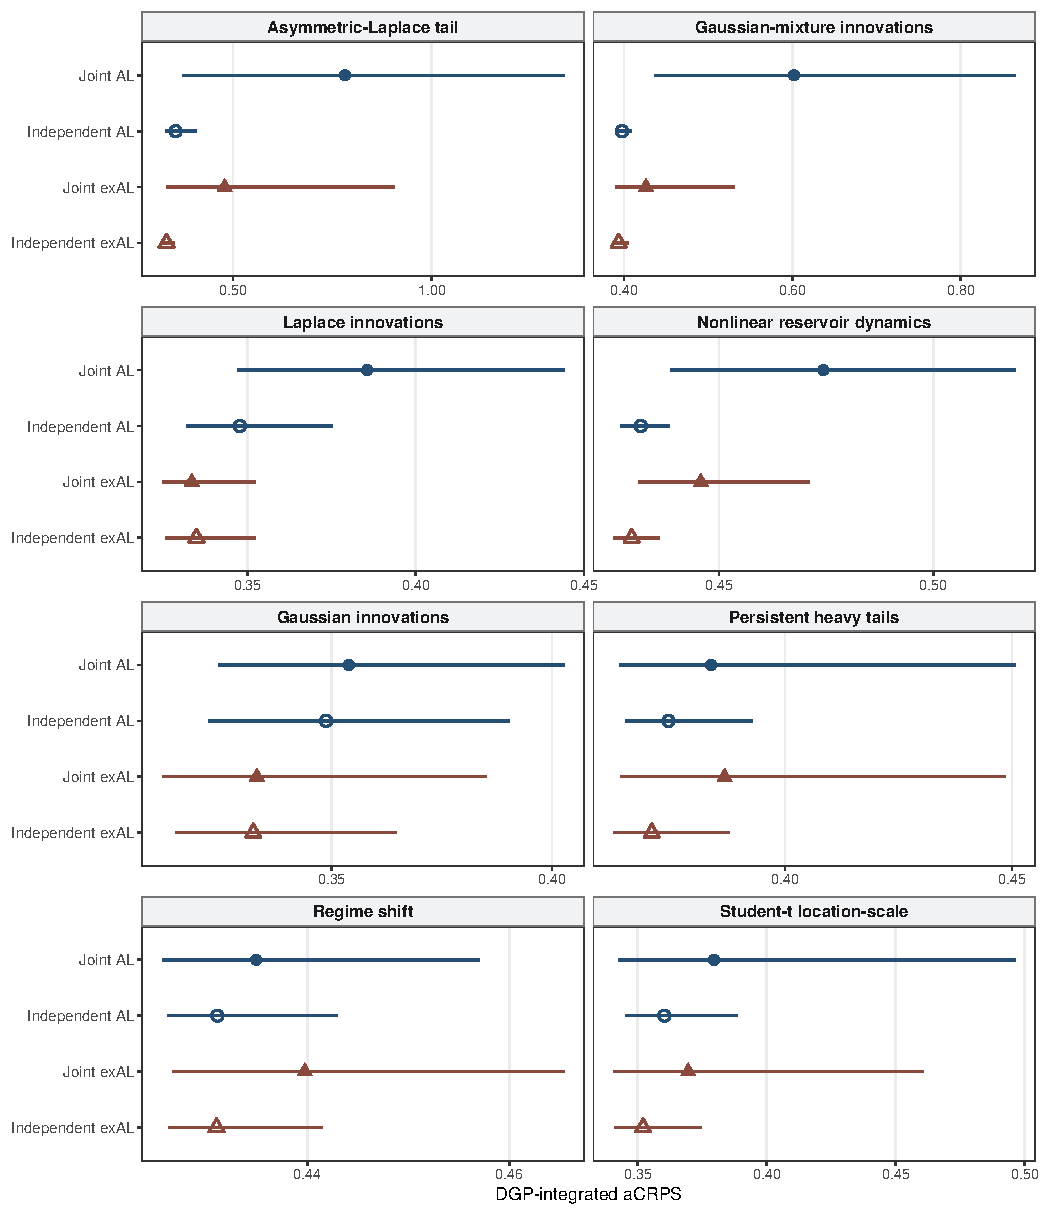
\includegraphics[width=0.94\textwidth]{figures/ch04-qdesn/joint_qdesn_simulation/joint_qdesn_corrected_v4_forecast_dgp_acrps.pdf}
\caption{Corrected posterior DGP-integrated \(\aCRPS\) for the joint multi-quantile study. Colored points are posterior means and horizontal segments are equal-tailed 95\% intervals. Lower values are better. Filled symbols denote joint fits, open symbols independent fits, blue \(\AL\), and red \(\exAL\). Marginal intervals for the numerical winner and runner-up overlap in every setting. Crossing frequencies and monotone-adjustment magnitudes are reported in the integrated technical material.}
\label{qdesn:fig:joint-qdesn-corrected-v4-forecast-acrps}
\end{figure}
